% Template Created by Mau Muñoz (https://github.com/maumchaves) following the
% specification for thesis documents provided by the Universitat Pompeu Fabra,
% Barcelona (https://guiesbibtic.upf.edu/tesis/eng/writing).

\documentclass{upfthesis}

\usepackage[utf8]{inputenc}

% TL;DR: Times-New-Roman-like font for Latex
% https://ctan.org/pkg/mathptmx
\usepackage{mathptmx}

% Can be changed according to your requirements
\usepackage[english]{babel}
\selectlanguage{english}

\usepackage{graphicx}
\graphicspath{ {images/} }

\usepackage{subcaption}

\usepackage{csquotes}

% Generates random content to fill this template
\usepackage{blindtext}
\usepackage{lipsum}

% Only (useful) for testing
\usepackage{showframe}

% Required only to style code snippets
\usepackage{listings}
\usepackage{color}
\definecolor{codebackcolor}{rgb}{0.95,0.95,0.92}
\lstdefinestyle{codestyle}{
    backgroundcolor=\color{codebackcolor},
    basicstyle=\footnotesize\ttfamily,
    breakatwhitespace=false,
    breaklines=true,
    keepspaces=true,
    showspaces=false,
    showstringspaces=false,
    showtabs=false,                  
    tabsize=4
}
\lstset{style=codestyle}

\usepackage{hyperref}

\title{UPF Thesis Template in \LaTeX{}}
\author{Mau Muñoz}
\date{July 2019}
% To update the date at the time you compile your document
% \date{\today}

\begin{document}

  \maketitle

  \begin{abstract}
  \lipsum[1]
\end{abstract}

  \tableofcontents
  \thispagestyle{empty}
  \clearpage

  \listoffigures
  \thispagestyle{empty}
  \clearpage

  \pagenumbering{arabic}

  \chapter{Handbook}
 
\section{Chapters}

\section{Paragraphs}

\section{Citation}

\section{Font Format}
 
Some of the \textbf{greatest} discoveries in \underline{science} were made by \textbf{\textit{accident}}. This is an \emph{emphasized} word inside normal text. \textit{And this is an \emph{emphasized} word inside an italicized text.}

\subsection{Bold}
\begin{lstlisting}
  \textbf{<your text>}
\end{lstlisting}

\subsection{Underline}
\begin{lstlisting}
  \underline{<your text>}
\end{lstlisting}

\subsection{Italic}
\begin{lstlisting}
  \textit{<your text>}
\end{lstlisting}

\subsection{Emphasis}
\begin{lstlisting}
  \emph{<your text>}
\end{lstlisting}
 
\section{Images and Figures}

\subsection{Baseline images}

Lorem ipsum dolor sit amet, consectetur adipiscing elit. Suspendisse nec pellentesque nunc. Sed massa diam, gravida ut est sit amet, molestie viverra nunc. Nam id ex ut tortor viverra auctor. 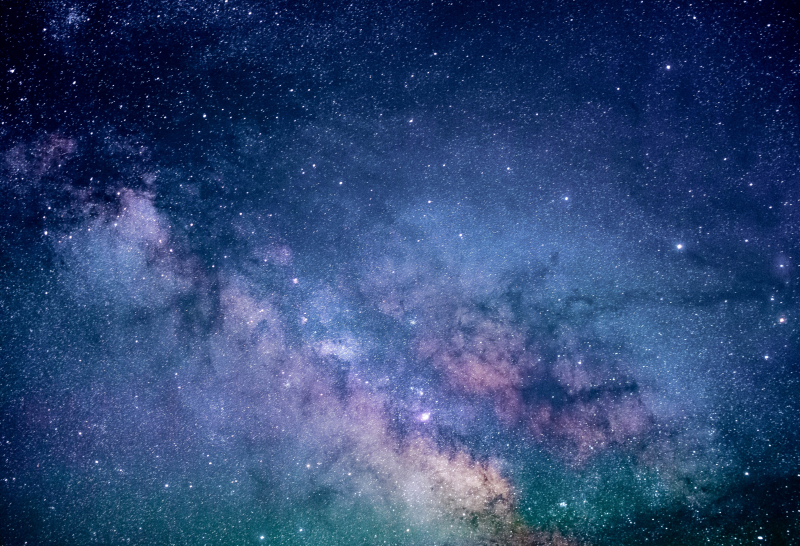
\includegraphics[height=\baselineskip]{image-1} Lorem ipsum dolor sit amet, consectetur adipiscing elit. Suspendisse nec pellentesque nunc. Sed massa diam, gravida ut est sit amet, molestie viverra nunc. Nam id ex ut tortor viverra auctor. 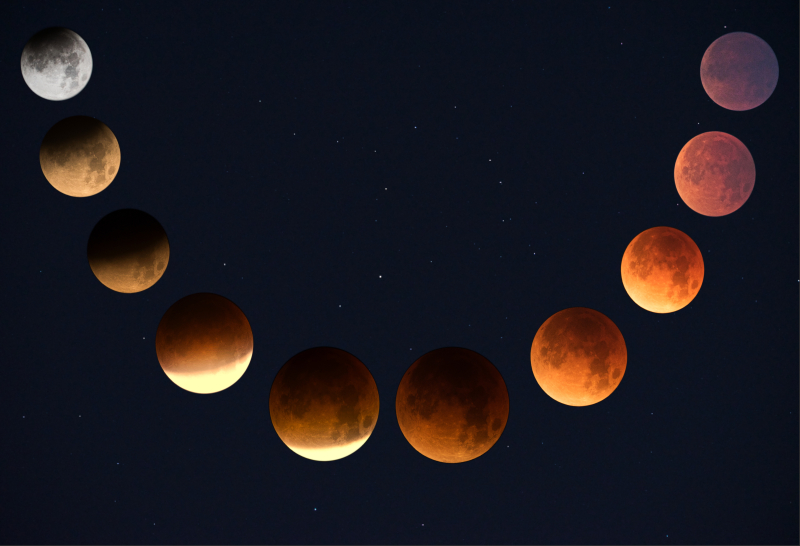
\includegraphics[height=\baselineskip]{image-2}.

\begin{lstlisting}
  \includegraphics[height=\baselineskip]{<file-name>}
\end{lstlisting}

\clearpage
\subsection{Full width image}

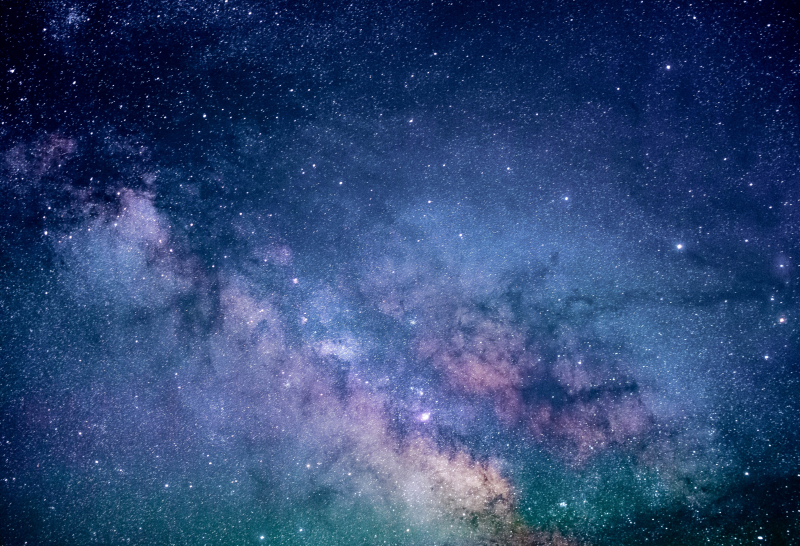
\includegraphics[width=\linewidth]{image-1}

\begin{lstlisting}
  \includegraphics[width=\linewidth]{<file-name>}
\end{lstlisting}

\clearpage
\subsection{Image with specific height}

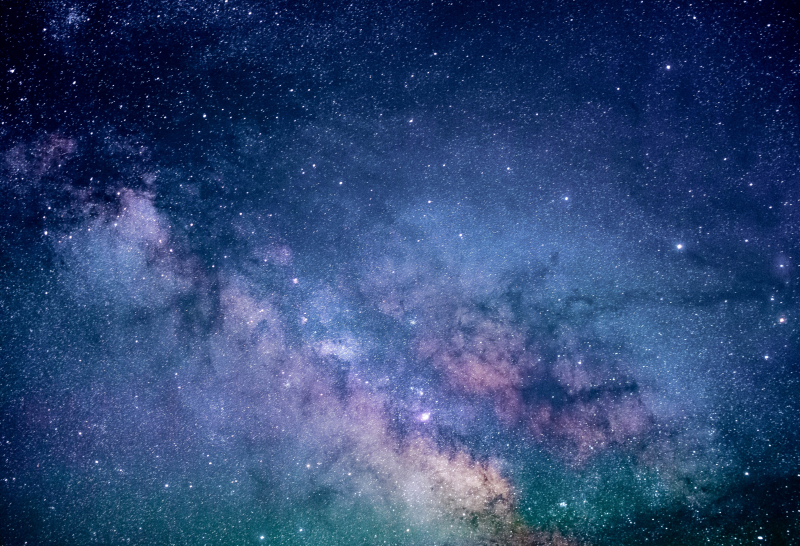
\includegraphics[height=3cm]{image-1}

\begin{lstlisting}
  \includegraphics[height=3cm]{<file-name>}
\end{lstlisting}

\clearpage
\subsection{Grid of images}

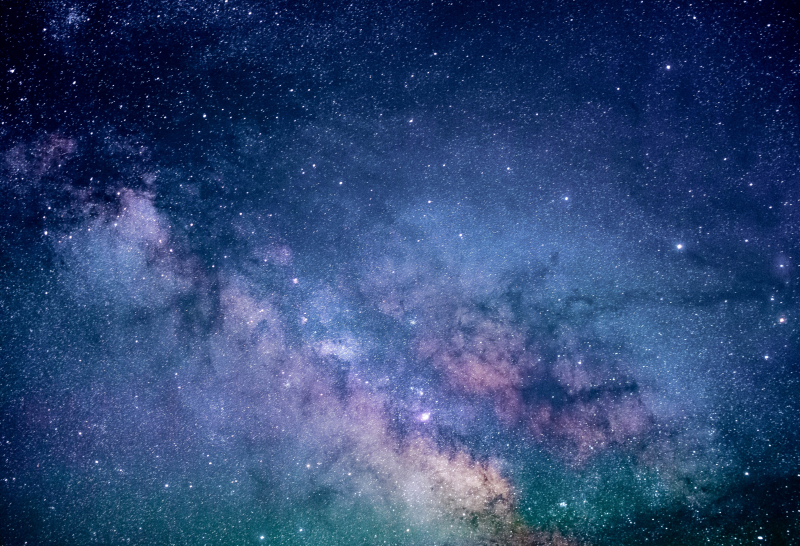
\includegraphics[width=0.3\linewidth]{image-1}
\quad
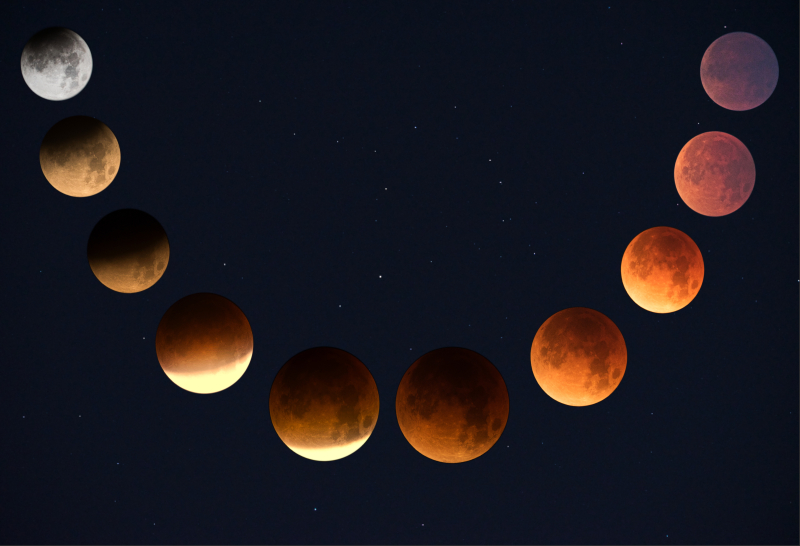
\includegraphics[width=0.3\linewidth]{image-2}
\quad
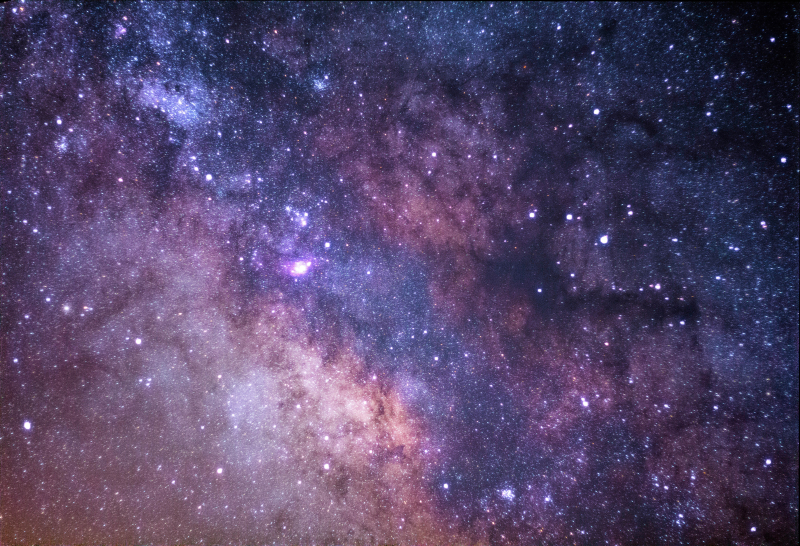
\includegraphics[width=0.3\linewidth]{image-3}
\\[\baselineskip]% adds vertical line spacing
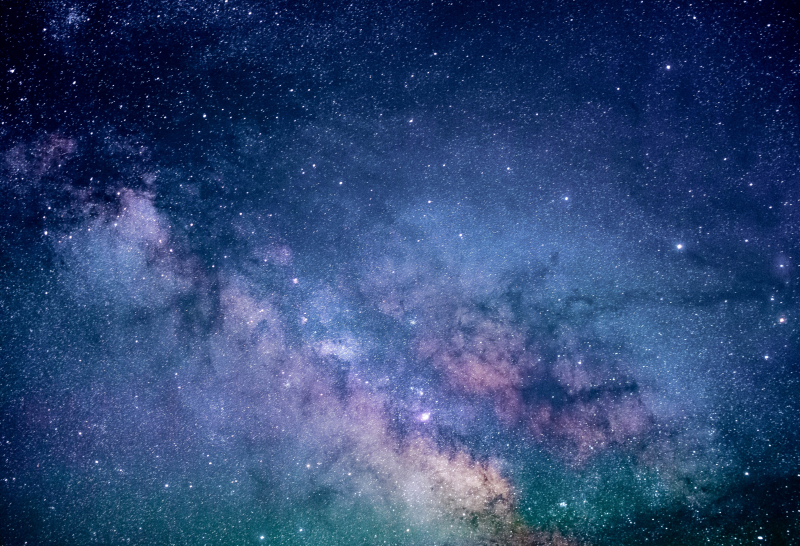
\includegraphics[width=0.3\linewidth]{image-1}
\quad
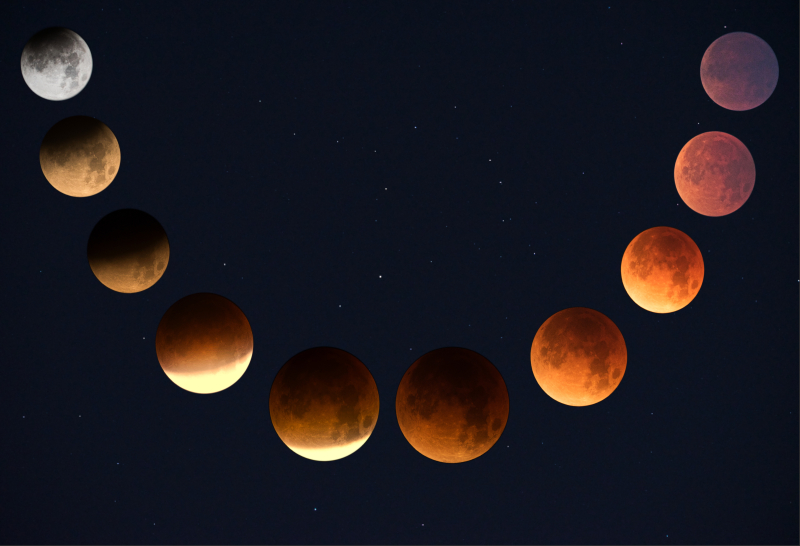
\includegraphics[width=0.3\linewidth]{image-2}
\quad
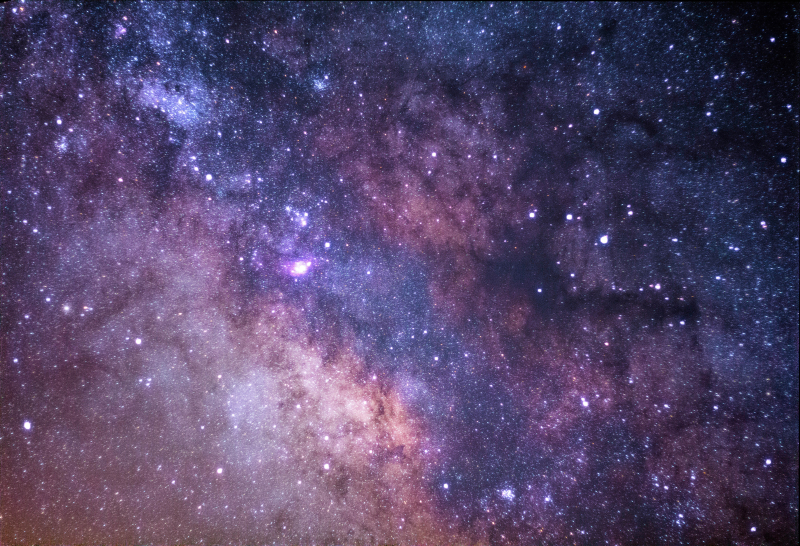
\includegraphics[width=0.3\linewidth]{image-3}

\begin{lstlisting}
  % first column
  \includegraphics[width=0.3\linewidth]{<file-name>}
  \quad % adds horizontal line spacing
  \includegraphics[width=0.3\linewidth]{<file-name>}
  \quad
  \includegraphics[width=0.3\linewidth]{<file-name>}

  \\[\baselineskip] % adds vertical line spacing

  % second column
  \includegraphics[width=0.3\linewidth]{<file-name>}
  \quad
  \includegraphics[width=0.3\linewidth]{<file-name>}
  \quad
  \includegraphics[width=0.3\linewidth]{<file-name>}
\end{lstlisting}

\clearpage
\subsection{Centered Figure}

\begin{figure}[h]
  \centering
  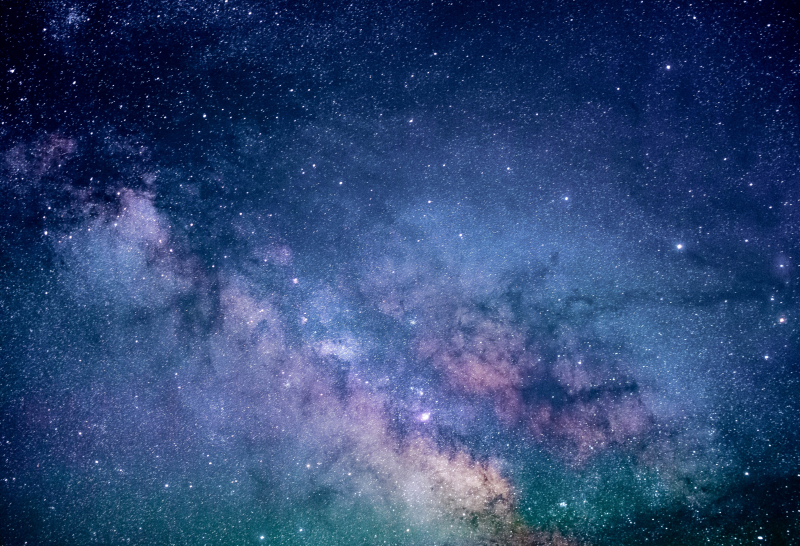
\includegraphics[width=0.5\textwidth]{image-1}
  \caption{This is a centered figure}
  \label{fig:image1}
\end{figure}

\begin{lstlisting}
  \begin{figure}[h]
    \centering
    \includegraphics[width=0.5\textwidth]{<file-name>}
    \caption{This is a centered figure}
    \label{fig:<yourFigureLabel>}
  \end{figure}
\end{lstlisting}

\clearpage
\subsection{Grid of figures}

\begin{figure}[h]
  \centering
  \begin{subfigure}{0.45\textwidth}
    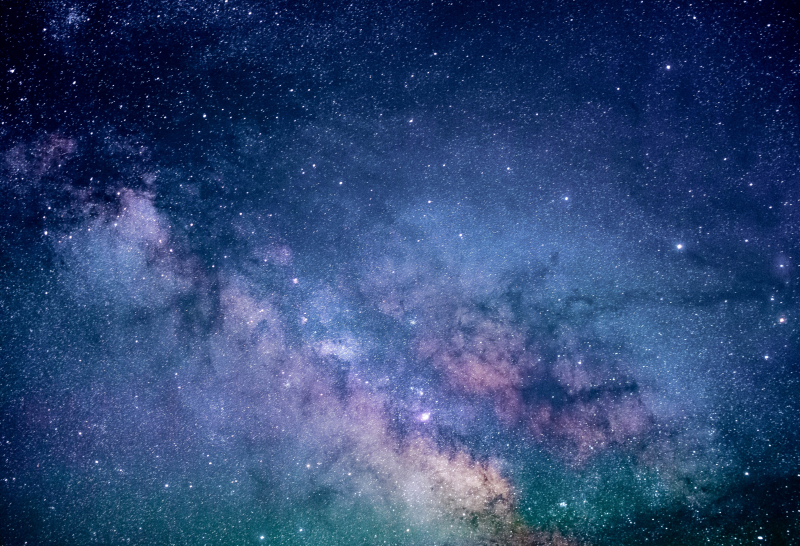
\includegraphics[width=\linewidth]{image-1} 
    \caption{Caption subfigure 1}
    \label{fig:subim1}
  \end{subfigure}%
  \quad
  \begin{subfigure}{0.45\textwidth}
    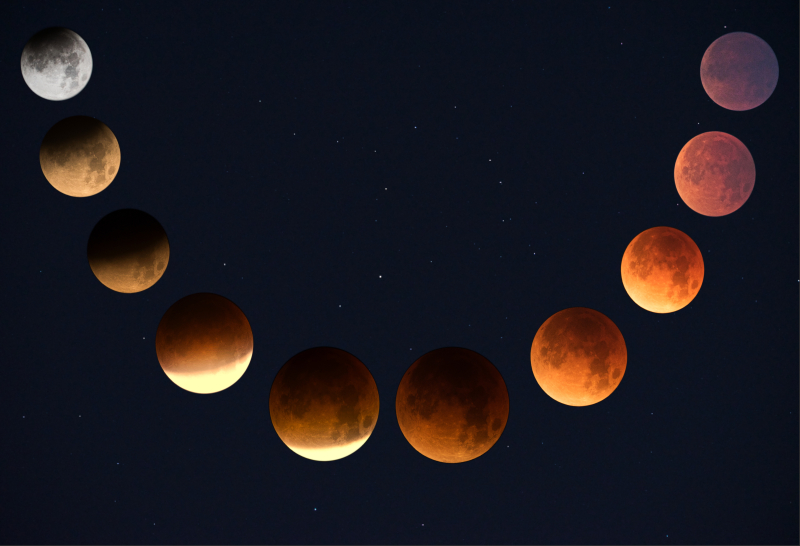
\includegraphics[width=\linewidth]{image-2}
    \caption{Caption subfigure 2}
    \label{fig:subim2}
  \end{subfigure}%
  \caption{This is a grid of figures with two images}
  \label{fig:image2}
\end{figure}

\begin{lstlisting}
  \begin{figure}[h]
    \centering
    \begin{subfigure}{0.45\textwidth}
      \includegraphics[width=\linewidth]{<file-name>} 
      \caption{Caption subfigure 1}
      \label{fig:<yourSubigureLabel>}
    \end{subfigure}%
    \quad
    \begin{subfigure}{0.45\textwidth}
      \includegraphics[width=\linewidth]{<file-name>}
      \caption{Caption subfigure 2}
      \label{fig:<yourSubigureLabel>}
    \end{subfigure}%
    \caption{This is a grid of figures with two images}
    \label{fig:<yourFigureLabel>}
  \end{figure}
\end{lstlisting}
  \chapter{Example}
 
\section{Introduction}
 
% Remove the `\lipsum` random text generator and place your content
\lipsum[1]
 
\section{Second Section}
 
\lipsum[1]
 
\subsection{First Subsection}

\lipsum[1]

\subsubsection{Subsubsection}

\lipsum[1]
 
\section*{Unnumbered Section}

\lipsum[1]

\textbf{Reference a figure:}

You can reference the figure \ref{fig:image1}. Also, you can reference the page \pageref{fig:image1} where the figure is.

\textbf{Unordered lists:}

\begin{itemize}
  \item The individual entries are indicated with a black dot, a so-called bullet.
  \item The text in the entries may be of any length.
\end{itemize}

\textbf{Ordered lists:}

\begin{enumerate}
  \item The individual entries are indicated with a black dot, a so-called bullet.
  \item The text in the entries may be of any length.
  \item \blindtext
\end{enumerate}

\textbf{Aligned text:}
\begin{center}
  Example 1: This text is an example of Center Alignment using the center environment. You can also use \verb|flushleft| and \verb|flushright|.
\end{center}

\textbf{New Paragraph:}
This is the text in first paragraph. This is the text in first paragraph. This is the text in first paragraph. \par
This is the text in second paragraph. This is the text in second paragraph. This is the text in second paragraph.
\\ % break line: starts a new line (also `\newline`).
This is the text in second paragraph. This is the text in second paragraph. This is the text in second paragraph.

\begin{verbatim}
  \textbf{New Paragraph:}
\end{verbatim}

\end{document}